\chapter{Präzisierung der Aufgabenstellung}\label{chap:Präzisierung_der_Aufgabenstellung}


Um herauszufinden, bei welchem Detektor die Güte am höchsten ist, lohnt es sich zunächst das Prozessbild aus dem Stand der Technik zu \ref{fig:Prozessbild_erw} zu erweitern . Die in der Literatur vorgeschlagenen Detektoren sind hier auf der Höhe der Annotationsunterstützungssoftware und des medizinischen Personals dargestellt, da Sie deren Aufgaben ganz oder teilweise übernehmen sollen. 

Da die Detektoren eine sehr unterschiedliche Funktionsweise haben können, müssen die Detektoren anhand ihrer Ergebnisse untereinander verglichen werden. Dies kann jedoch nicht zu qualitativen Aussagen führen, da nicht entschieden werden kann, welche Beinbewegungen als richtig annotiert gelten. Aus diesem Grund werden die Ergebnisse paarweise mit den Ergebnissen den medizinischen Fachpersonals verglichen. Da aus dem Annotationssignal die Kennwerte berechnet werden, bieten sich diese zusätzlich als Vergleichsmöglichkeit in der Datenverarbeitungskette an.
Dieses Vorgehen hat den zusätzlichen Vorteil, dass auch Detektoren untereinander verglichen werden können, welche andere Eingangssignale nutzen. Hierzu zählen: Videoanalyse \cite{robust}, Aktigramm \cite{PDS}, Kraftsensoren unter der Matratze \cite{Kraft}, Bioimpedanzänderung bei Bewegung \cite{Mehrkanal-BioimpedanzInstrumentierung}, Elektrocardiogramm \cite{cardio}, Flugzeitsensoren \cite{timeofflight}. 


\begin{figure}[!ht]%
	\begin{center}
	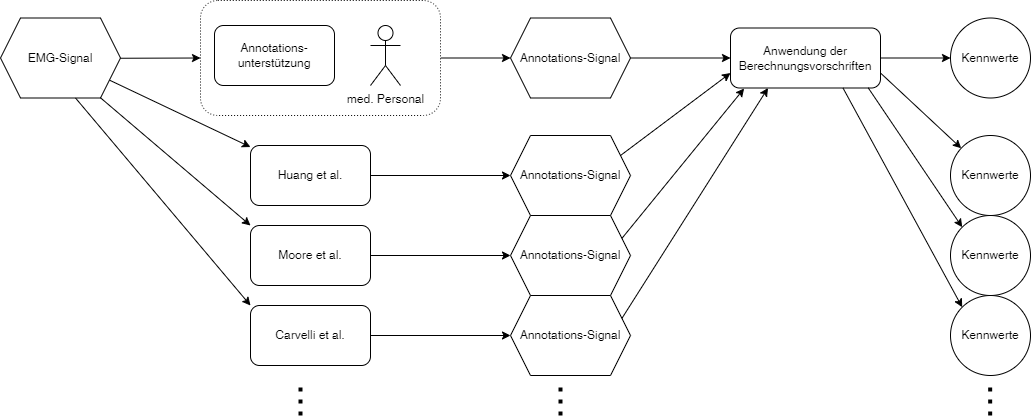
\includegraphics[width=0.80\textwidth]{./Bilder/Prozessbildrot_erweitert.drawio (1).png}
	\end{center}
	\caption{Erweiterte Datenverarbeitungskette aus \ref{fig:Prozessbild} zur Veranschaulichung der Vergleichsmöglichkeiten}%
	\label{fig:Prozessbild_erw}%
\end{figure}
\newpage
Als Metrik wird hier ein skalarer Wert definiert, mit dem Detektoren Verglichen werden können.
Aus den oben genannten Problemen ergibt sich die dringende Notwendigkeit, eine Metrik zu finden, welche 
\begin{enumerate}
	\item Einfache, einheitliche und eindeutige Vergleichbarkeit zwischen Detektoren ermöglichen,
	\item die Güte in dem medizinischen Kontext bewerten und 
	\item benutzt werden können, um Detektoren zu verbessern.
\end{enumerate}

In der folgenden Arbeit sollen diese Probleme gelöst werden.
Die AASM ist sich dieser Problematik bewusst und arbeitet daran Metriken zu untersuchen \cite{comingsoon}. 
